\documentclass[10pt,a4,oneside]{article}
\usepackage{a4wide}
\usepackage{graphicx}

\begin{document}
\begin{titlepage}
\begin{center}

\includegraphics[width=40mm]{figs/earth}
\vfill
\textbf{\huge Milestone 3 Plan}\\ \textit{} \\ \textit{} 
\textit{for} \\ \textit{} \\ \textit{} 
\textbf{\huge Team 1}\\ \textit{} \\ \textit{}
\vfill
\textbf{Alex Egan \\ Filimoni Lutunaika \\ George Sainsbury \\ Xiaodong Cui}
\end{center}
\end{titlepage}
 


\newpage

\tableofcontents

\[----\]

\paragraph{}

\listoffigures
 
\newpage

\section{Introduction} 
 
\subsection{Purpose and Scope}

\label{subsec:purpose-and-scope}
 
Milestone 3 follows on from the development tasks undertaken during Milestones 1 and 2.
Team 1 is investigating the following 3 tickets during the current development sprint:

\subsubsection*{Ticket 131 - Use real disk usage instead of byte size throughout the web application}

\noindent Information of disk space usage is being gathered by the Earth application.
This is a better and more precise metric for determining where disk space 
is used. The GUI should be able to use this value instead in all situations. 

\subsubsection*{Ticket 148 - Configuration of daemon should be possible through GUI}

\noindent The daemon configuration options should be done through the 
administrative interface of Earth so that starting a daemon on a server 
is as simple as ./earth\_daemon.rb and all options are fed from a central 
location.

\noindent Of course, this has implications that we should be able to add 
a server to be indexed through the admin interface instead of it being 
created the first time the daemon runs. 


\subsubsection*{ Ticket 174 - Look into making Earth release a gem}

\noindent It would allow us to automatically deal with the dependencies such as:

\begin{itemize}
\item the gems:
  \subitem rcov
  \subitem rails
  \subitem postgres 
\end{itemize}
 
\noindent The remove feature of the daemon is also being considered by Team 1 for Milestone 3. 

 
\subsection{Plan Review}
 
\noindent This plan will be reviewed at the end of the Milestone 3 development 'sprint'. This plan 
will be updated if there is a radical change to the requirements of any Milestone 3 task. 
The changes can be made by any of the team member who should then inform the team leader 
about these changes. However, significant changes that have a system-wide effect will be deferred 
to the next milestone to minimize any disruption to the other tasks of the current milestone.

\newpage

\section{Organisation for Milestone 3}
 
\label{sec:g1org}

\subsection{Task Allocations}

Tasks for Milestone 3 are being allocated as follow:
 
\subsubsection{Ticket 131: Use real disk usage instead of byte size}

\paragraph{Description}
Cui has been allocated this Ticket given its priority and the 
importance of real disk usage information for the Earth application. 
Given the vague description for this ticket on the Trac system,
the task has been further sub-divided into subtasks to allow for
better allocation of resources and proper monitoring.

\paragraph{Subtasks}
\noindent
\begin{enumerate}
\item Need to find the how files are stored in the disk, how much 
disk space must be used to store a given size file, then the relationship 
between the file size and actual disk space. (10hrs)
\item Change the byte size to real disk usage. (15hrs)
\item Use the real disk usage in all web applications. (15hrs)
\item Integration Testing (10hrs)
\end{enumerate}

\paragraph{Total Time Estimate} 50hrs


\subsubsection{Ticket 148: Configuration of Daemon using GUI}

\paragraph{Description}
Fil is being allocated this task for Milestone 3 to allow for the 
easy re-configuration of the earthd daemon when switching between 
the three operating modes of the application: development, test 
and production. This feature is particularly useful during the 
integration testing phase where regular switching between the 
various operating modes will be required.

\paragraph{Subtasks}
\noindent
\begin{enumerate}
\item Identify all current and available configuration options for the Earth daemon. (5hrs)
\item Design page layout and select appropriate control options such as textboxes and buttons. (15hrs)
\item Implement scripts linking page controls and daemon features. (20hrs)
\item Integration Testing (10hrs)
\end{enumerate}

\paragraph{Total Time Estimate} 50hrs
 

\subsubsection{Ticket 174: Creating the Earth Gem}

\paragraph{Description}
George is being allocated this task which involves investigating 
the process of creating the Earth Gem. The availability of this 
Gem will have a significant impact on the productivity of developers 
as less resources (time) is required to re-installing the Earth
application.

\paragraph{Subtasks}
\noindent
\begin{enumerate}
\item Identify all dependencies for the basic Earth installation (4hrs)
\item Investigate the process of creating a gem of the Earth application (16hrs)
\item Integration Testing (4hrs)
\end{enumerate}

\paragraph{Total Time Estimate} 24hrs
 
\subsubsection{Earth Feature: Investigate Implementation of the Daemon Remove Function}

\paragraph{Description}
Alex is being allocated this task which entails investigating the implementation of the 
Earth application remove function. This is certainly a non-trivial task that the Team 
has decided to investigate during this development sprint.

\paragraph{Subtasks}
\noindent
\begin{enumerate}
\item Conduct exploratory study of ways to implement the Earth remove function (12hrs)
\item Document feasibility of each identified implementation approach (8hrs)
\item Integration Testing (4hrs)
\end{enumerate}

\paragraph{Total Time Estimate} 24hrs

\newpage
 
\subsection{Scheduling}

\paragraph{} 
The milestones and tasks are shown graphically in Figure \ref{fig:m3gantt} below. 
This figure shows the relative times between the deadlines of the tasks required 
and also shows the estimated time for the completion of each individual tasks.
 
\begin{figure}[h!]
\begin{centering}
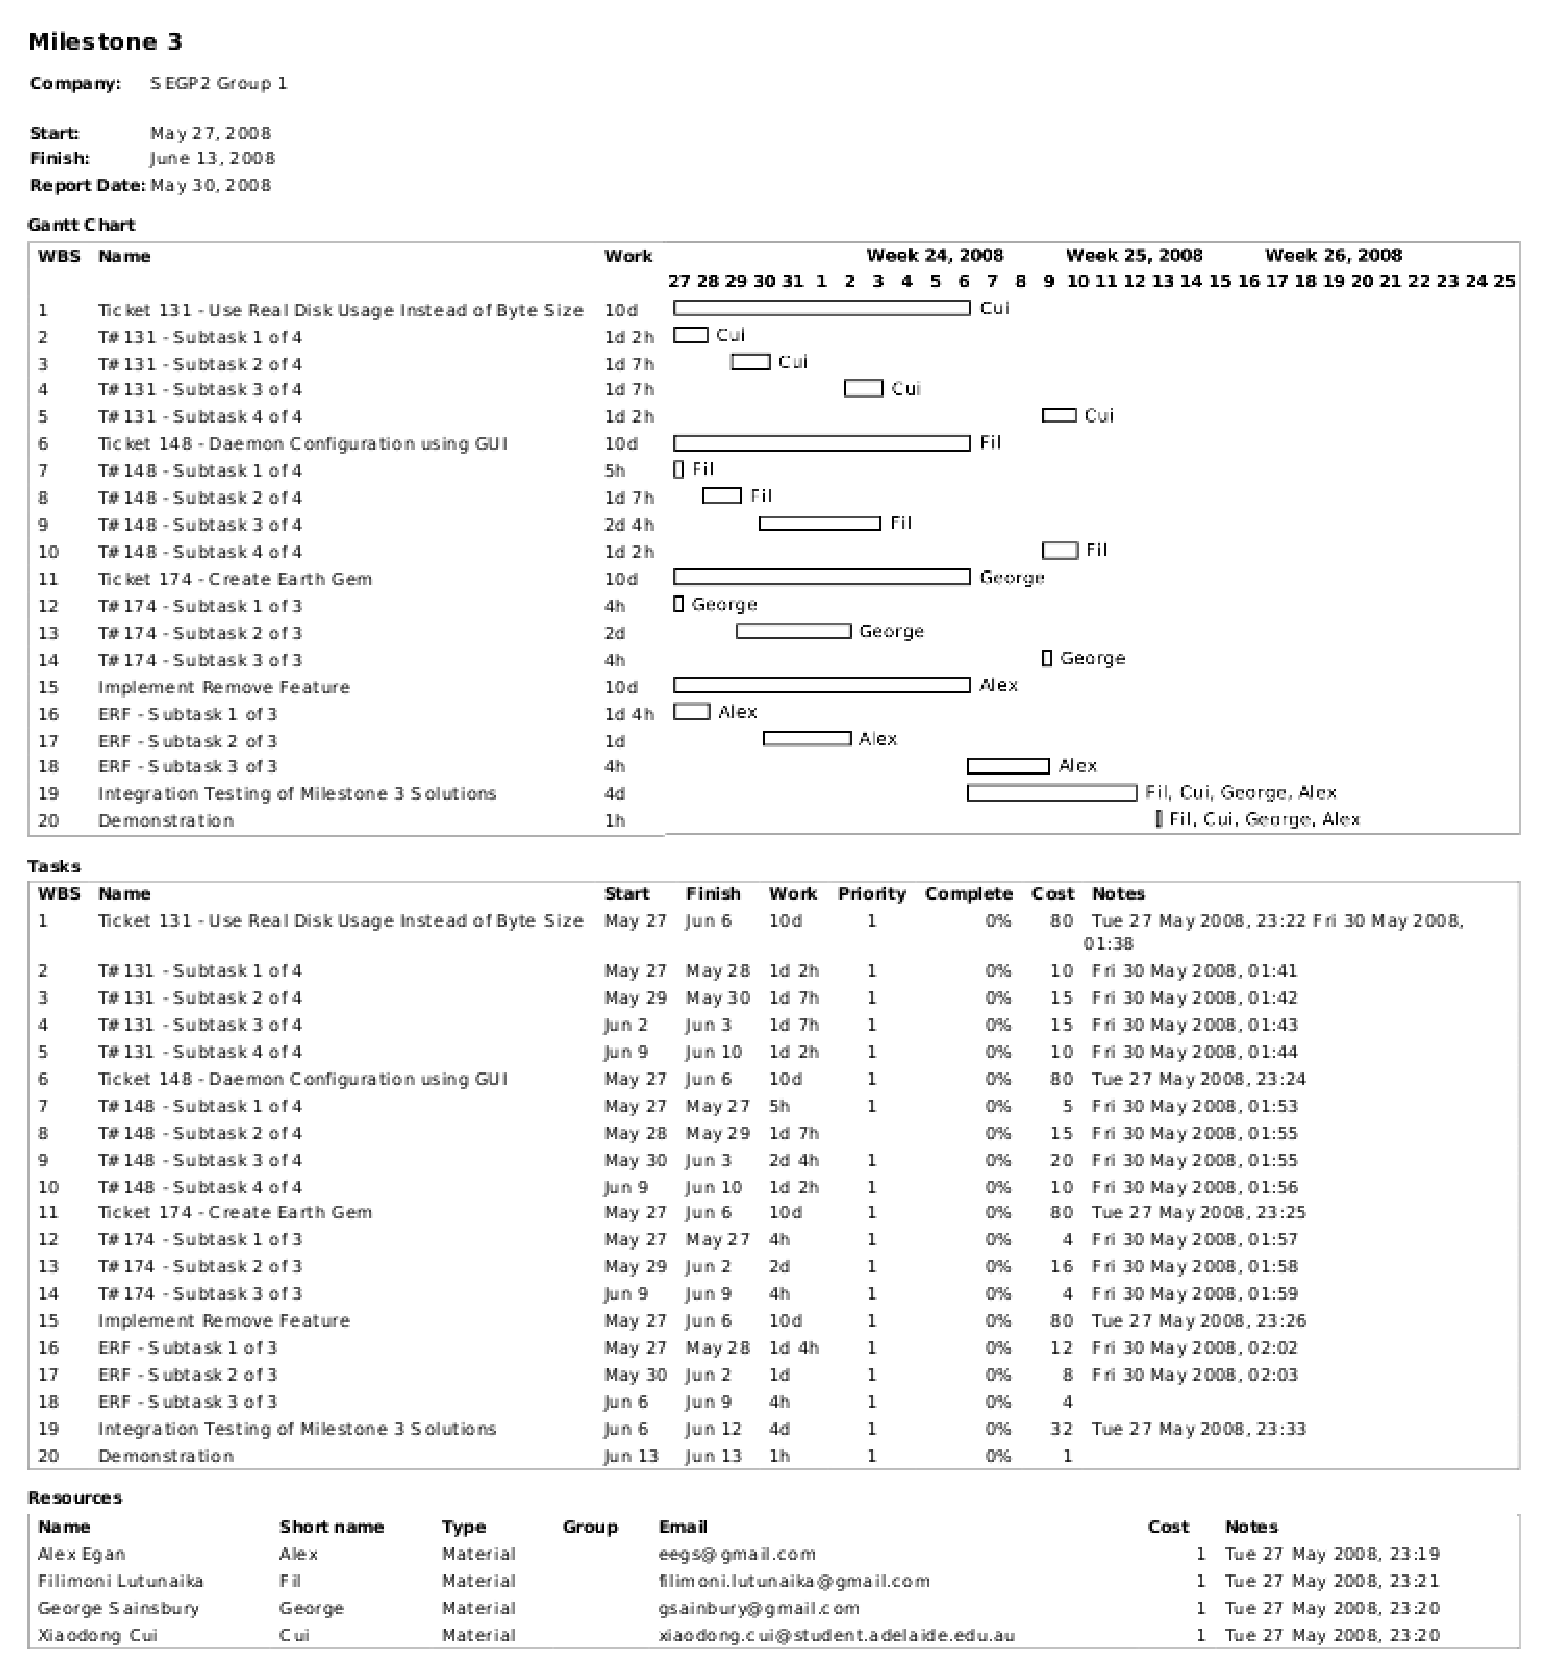
\includegraphics[width=150mm]{figs/m3gantt}
\end{centering}
\caption{Gantt chart of tasks for milestone 3}
\label{fig:m3gantt}
\end{figure}

\newpage

\subsection{Resource Allocation}
 
\paragraph{}
As described in Section \ref{subsec:purpose-and-scope}, resources (developers) will be allocated to 
each task as follow:
 
\begin{itemize}
  
\item \textbf{Ticket 131:} Xiaodong Cui \\
 
\item \textbf{Ticket 148:} Filimoni Lutunaika \\
 
\item \textbf{Ticket 174:} George Sainsbury \\
 
\item \textbf{Earth Remove Feature:} Alex Egan \\
 
\end{itemize}
 
If a task is completed early, or it is noted that less people are required to complete a task on schedule, they will be reallocated to other tasks.\\
 

\subsection{Source Control}

\subsubsection{Task Completion Criteria}

\noindent To ensure the successful integration of each allocation tasks into the team repository, the member responsible will have to make sure that at least one of the other team members can successfully duplicate the end results or outcome of the task.

\paragraph{}
\noindent Upon satisfying the above requirement, the member responsible can then make a pull request to the team's gitHub leader to upload the solution onto the team's git repository for the actual integration testing of the team's collective solutions. 


\subsubsection{Git Repository Process}

\noindent Each team member is expected to follow the git repository procedures outlined in the \emph{Repository Process Document for Earth}.
 

\subsubsection{Testing Process}
\noindent Each team member is expected to follow the testing process procedures outlined in the \emph{Testing Process Document for Earth}.


\subsection{Administration}

In addition to the assigned tasks for this Milestone 1, the roles of Git Leader and Documentation Person will be rotated amongst the Team 1 members at every milestone. This will help to ensure that each member gets a chance to take on extra responsibilities with the view of broadening their individual skills as a software developer.

\subsubsection{Git Leader}

For Milestone 3, Alex will be in charge of managing the repository for Team 1. This includes ensuring that the Milestone 3 solutions undergo integration testing before being committed onto the Team 1 repository.


\subsubsection{Documentation Person}

For Milestone 3, Fil will oversee the documentation requirements for Team 1, which mainly includes setting meeting agendas and organising progress update meetings.

\newpage

\section{References}
 
Sommerville, I. \textit{Software Engineering}, 8th Edition,  Addison-Wesley, 2007\\
\newline
Wikipedia, \textit{Agile software development} Retrieved from \emph{http://en.wikipedia.org/wiki/Agile\_software\_development} on 27/05/2008.\\
\newline
Earth Project, \textit{Ticket 138} Retrieved from \emph{http://open.rsp.com.au/projects/earth/ticket/138} on 27/05/2008.\\
\newline
Earth Project, \textit{Ticket 148} Retrieved from \emph{http://open.rsp.com.au/projects/earth/ticket/148} on 27/05/2008.\\
\newline
Earth Project, \textit{Ticket 174} Retrieved from \emph{http://open.rsp.com.au/projects/earth/ticket/174} on 27/05/2008.\\
\newline
Egan, A and Bamogaddam, M.,\textit{Testing Process Document for Earth} Egan, A and Bamogaddam, M., First Edition, 2008.\\
\newline
Egan, A and Bamogaddam, M.,\textit{Repository Process Document for Earth}  First Edition, 2008.\\

\paragraph{}

\[ END\]
\end{document}
